% Made up for the tikra benchmark.
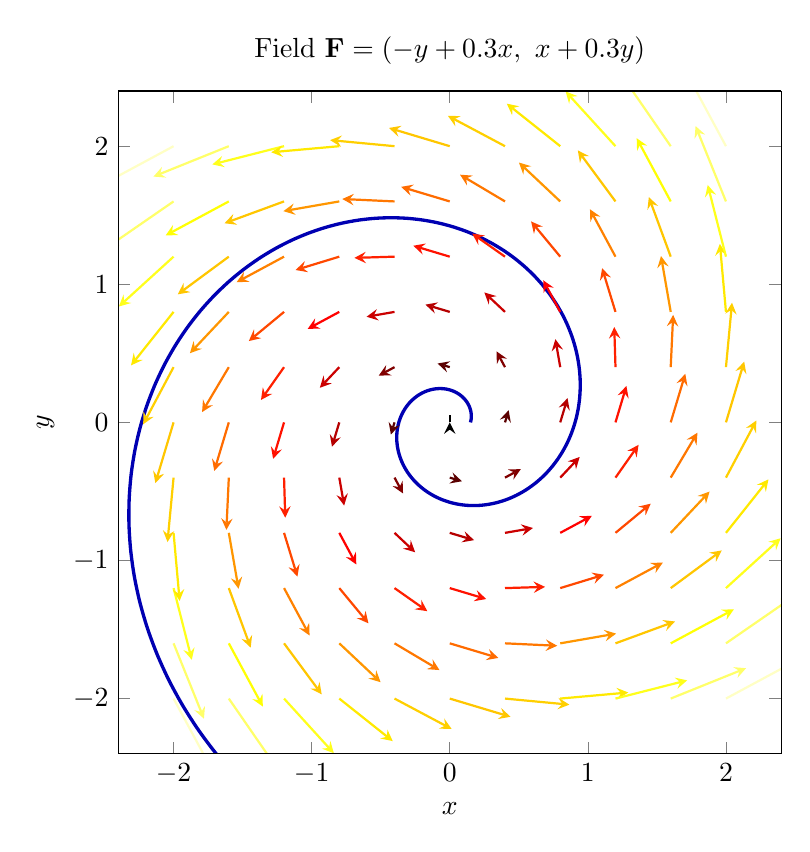
\begin{tikzpicture}
\begin{axis}[width=10cm, height=10cm, axis equal image, xmin=-2.4, xmax=2.4, ymin=-2.4, ymax=2.4,
    xlabel=$x$, ylabel=$y$, title={Field $\mathbf{F} = (-y + 0.3x,\ x + 0.3y)$},
    colormap/hot2, point meta min=0, point meta max=3, view={0}{90}]
  \addplot[blue!70!black, very thick, domain=0:620, samples=150, variable=\t, smooth]
    ({0.15*exp(0.005*\t)*cos(\t)}, {0.15*exp(0.005*\t)*sin(\t)});
  \addplot3[point meta={sqrt(x^2+y^2)}, quiver={u={-y + 0.3*x}, v={x + 0.3*y}, w=0, scale arrows=0.22,
      every arrow/.append style={-stealth, line width=0.8pt, color=mapped color}},
      samples=11, domain=-2:2, y domain=-2:2] (x, y, 0);
\end{axis}
\end{tikzpicture}
